\documentclass{article}

\usepackage{amssymb, amsmath, amsfonts}
\usepackage{amsthm}
\usepackage{tikz}
\usetikzlibrary{matrix, shapes,arrows}
\usepackage{pgfplots}
\usepackage[a4paper, margin=1in]{geometry}

\newtheorem{proposition}{Proposition}
\newtheorem{theorem}{Theorem}
\newtheorem{definition}{Definition}
\newtheorem{lemma}{Lemma}
\newtheorem{conjecture}{Conjecture}
\newtheorem{corollary}{Corollary}
\newtheorem{remark}{Remark}
\newtheorem{assumption}{Assumption}

\newlength\figureheight
\newlength\figurewidth

\newcommand{\tikzdir}[1]{tikz/#1.tikz}
\newcommand{\inputtikz}[1]{\tikzsetnextfilename{#1}\input{\tikzdir{#1}}}

\DeclareMathOperator*{\argmin}{arg\; min}     % argmin
\DeclareMathOperator*{\argmax}{arg\; max}     % argmax
\DeclareMathOperator*{\tr}{tr}     % trace
\DeclareMathOperator{\Cov}{Cov}
\DeclareMathOperator{\logdet}{log\;det}

\title{EE3011 Modeling and Control\\Tutorial 7: Frequency Responses}
\date{}
\begin{document} \maketitle

\begin{enumerate}
\item Consider the unity-feedback system with the open-loop transfer function  
  \[
    G(s) = \frac{10}{s+11}.
  \]
  Obtain the steady-state output of the system when it is subjected to each of the following inputs:
  \begin{enumerate}
  \item  $r(t) = \sin(t+30^\circ)$,
  \item  $r(t) = 2\cos(2t-45^\circ)$,
  \item  $r(t) = \sin(t+30^\circ)-2\cos(2t-45^\circ)$.
  \end{enumerate}

\item Calculate the magnitude and phase of the following transfer function at the frequency of $3\,rad/s$:
  \begin{enumerate}
  \item \[G_1(s) = 10\frac{s-1}{s+1},\]
  \item  \[G_2(s) = 10\frac{s^2-1}{s^2(s+1)}.\]
  \end{enumerate}

\item Find the magnitude and phase responses of the following transfer function
  \[
    G(s) = \frac{1}{(s+1)(s^2+s+1)}.
  \]
  Compute the steady-state responses to sinusoid $r(t) = 2\sin(\omega t+30^\circ)$ with frequency $\omega = 0.1,\,1,\,10\,rad/s$ respectively. Explain the results.

\item A control system for a flexible structure is shown in Figure~\ref{fig:sys} where is an output disturbance due to an external vibration source. Evaluate the attenuation for disturbance with frequency $1\,rad/s$ and $100\,rad/s$, respectively.
  \begin{figure}[ht]
    \centering
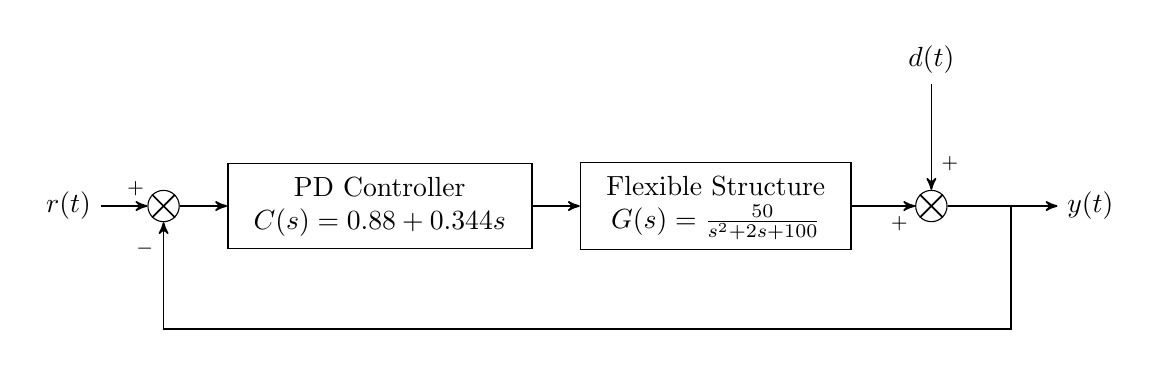
\begin{tikzpicture}[>=stealth',
box/.style={rectangle, draw, semithick},
point/.style={coordinate},
]
\matrix[row sep = 10mm, column sep = 6mm]{
&
&
&
&
\node (p) [] {$d(t)$};&
&\\
%first row
\node (p1) [] {$r(t)$};&
\node (p2) [circle,draw,inner sep=4pt] {};&
\node (control) [box] {\begin{tabular}{c}
                         PD Controller\\
                         $C(s)=0.88+0.344s$
                       \end{tabular}};&
                     \node (plant) [box] {\begin{tabular}{c}
                                            Flexible Structure\\
                                            $G(s)=\frac{50}{s^2+2s+100}$
                                          \end{tabular}};&

\node (p7) [circle,draw,inner sep=4pt] {};&
\node (p3) [point] {};&
\node (p4) [] {$y(t)$};\\
%second row
&
\node (p5) [point] {};&
&
&
&
\node (p6) [point] {};&\\
};
\draw [semithick,->] (p1)--node[near end, above]{\scriptsize{$+$}} (p2);
\draw [semithick,->] (p2)--(control);
\draw [semithick,->] (control)--(plant);
\draw [semithick,->] (plant)--node[near end,below]{\scriptsize{$+$}}(p7);
\draw [semithick,->] (p7)--(p4);
\draw [semithick,->] (p3)--(p6)--(p5)--node[near end, left]{\scriptsize{$-$}} (p2);
\draw [semithick] (p2.north east)--(p2.south west);
\draw [semithick] (p2.south east)--(p2.north west);
\draw [semithick] (p7.north east)--(p7.south west);
\draw [semithick] (p7.south east)--(p7.north west);
\draw [semithick,->] (p)--node[near end,right]{\scriptsize{$+$}}(p7);
\end{tikzpicture}
    \caption{\label{fig:sys} Block Diagram for Question 4.}
  \end{figure}
\end{enumerate}

\newpage

\section*{Answers:}
\begin{enumerate}
\item 
  \begin{enumerate}
  \item $0.905\sin(t-24.8^\circ)$,
  \item $1.79\cos(2t-55.3^\circ)$,
  \item $0.905\sin(t-24.8^\circ)-1.79\cos(2t-55.3^\circ)$.
  \end{enumerate}
\item \begin{enumerate}
  \item $10$, $36.9^\circ$,
  \item $3.51$, $-71.6^\circ$.
  \end{enumerate}
\item \begin{enumerate}
  \item $2\sin(0.1t+18.5^\circ)$,
  \item $1.414\sin(t-105^\circ)$,
  \item $0.002\sin(10t-228.5^\circ)$.
  \end{enumerate}
\item $3.27$dB attenuation for $1\,rad/s$ and $0.12$dB attenuation for $100\,rad/s$.
\end{enumerate}
\newpage
\section*{Detailed Solution:}

\begin{enumerate}
\item Notice that
  \begin{align*}
    j\omega + 11 = \sqrt{121+\omega^2}\angle \tan^{-1}(\omega/11).
  \end{align*}
  Therefore
  \begin{align*}
    G(j\omega) = \frac{10}{\sqrt{121+\omega^2}\angle \tan^{-1}(\omega/11)} = \frac{10}{\sqrt{121+\omega^2}}\angle -\tan^{-1}(\omega/11)
  \end{align*}
\begin{enumerate}
\item $r(t) = \sin(t+30^\circ)$, hence $\omega = 1$. 
  \begin{align*}
    G(j1) = \frac{10}{\sqrt{122}}\angle -\tan^{-1}(2/11) = 0.905\angle -5.19^\circ.
  \end{align*}
  Therefore, the output equals
  \begin{align*}
    0.905\times 1 \sin(t + 30^\circ-5.19^\circ) = 0.905\sin(t+24.8^\circ).
  \end{align*}
\item $r(t) = 2\cos(2t-45^\circ)$, hence $\omega = 2$. 
  \begin{align*}
    G(j1) = \frac{10}{\sqrt{125}}\angle -\tan^{-1}(1/11) = 0.894\angle -10.31^\circ.
  \end{align*}
  Therefore, the output equals
  \begin{align*}
    0.894\times 2 \cos(t - 45^\circ-10.31^\circ) = 1.79\cos(t-55.3^\circ).
  \end{align*}
\item Using the linearity property, we know the output is given by
 \begin{align*}
      0.905\sin(t+24.8^\circ)- 1.79\cos(t-55.3^\circ).
 \end{align*}
\end{enumerate}
\item \begin{enumerate}
  \item Notice that
    \begin{align*}
      j\omega -1 &= \sqrt{1+\omega^2}\angle(180^\circ- \tan^{-1}\omega),\\
      j\omega +1 &= \sqrt{1+\omega^2}\angle\tan^{-1}\omega.
    \end{align*}
    Therefore,
    \begin{align*}
     G_1(j\omega) = 10\angle (180^\circ -2\tan^{-1}\omega),
    \end{align*}
    and
    \begin{align*}
      G_1(j3) = 10\angle 36.9^\circ.
    \end{align*}
  \item Notice that
    \begin{align*}
      (j\omega)^2 -1 &= 1+\omega^2\angle 180^\circ,\\
      (j\omega)^2  &= \omega^2\angle 180^\circ,\\
      j\omega+1  &= \sqrt{\omega^2+1}\angle \tan^{-1}\omega.
    \end{align*}
    Therefore,
    \begin{align*}
      G_2(j\omega) = 10\frac{\sqrt{\omega^2+1}}{\omega^2}\angle -\tan^{-1}\omega,
    \end{align*}
    and
    \begin{align*}
      G_2(j3) = 3.51\angle -71.6^\circ.
    \end{align*}
  \end{enumerate}
\item 
  \begin{align*}
    G(0.1j)&=0.980-0.199j = 1\angle -11.5^\circ,\\
G(1j) &= -0.500-0.500j = 0.707\angle -135^\circ,\\
G(10j) &= 10^{-4}\times (-1.99+9.80j) = 1.00\times 10^{-3}\angle -258.5^\circ.
  \end{align*}
Therefore, the output will be given by
\begin{align*}
  2\times 1 \sin(0.1t +30^\circ - 11.5^\circ) = 2\sin(0.1t+18.5^\circ),\\
  2\times 0.707 \sin(1t +30^\circ - 135^\circ) = 1.414\sin(1t-105^\circ),\\
  2\times 10^-3 \sin(10t +30^\circ - 258.5^\circ) = 0.002\sin(10t-228.5^\circ).
\end{align*}
\item Notice that
\begin{align*}
  Y(s) = \frac{1}{1+C(s)G(s)}D(s) = H(s)D(s),
\end{align*}
where
\begin{align*}
  H(s) = \frac{1}{1+C(s)G(s)} = \frac{s^2+2s+100}{s^2+19.2s+144}.
\end{align*}
Therefore,
\begin{align*}
  H(1j) = 0.682-0.078j = 0.686\angle -6.49^\circ,
\end{align*}
and
\begin{align*}
  H(100j) = 0.972+0.169j = 0.986\angle 9.86^\circ.
\end{align*}
As a result, the system has a $-20\log\,0.686 = 3.27$dB attenuation for frequency $1\,rad/s$ and $-20\log\,0.986 = 0.12$dB attenuation for frequency $100\,rad/s$.




\end{enumerate}

\end{document}
%%% Local Variables:
%%% TeX-command-default: "Latexmk"
%%% End:
